\chapter{Prototype Design}

The objective of this project is to create and construct a prototype digital library catered specifically to Māori language users, addressing their requirements for book retrieval, borrowing, and return functionalities, while enhancing their overall library experience. The prototype library targets the global community of Maori speakers, encompassing Maori educators, students, parents, and the general learner.

The Maori language holds a significant position as one of the official languages of the indigenous Maori people in New Zealand, playing a crucial role in the cultural and social advancement of the country. With the aim of fostering the preservation and growth of the Maori language, the prototype digital library will offer a wide array of Maori language books to cater to the needs of Maori language users. This initiative aims to facilitate online reading and learning, making a meaningful impact on Maori language education and cultural enrichment heritage\cite{Discover30:online}.

\section{Design principles and methodology}

The design approach for the digital library prototype will adhere to the following guiding principles:

User-centricity: The project will prioritize the needs, preferences, and overall satisfaction of the users, ensuring the provision of efficient and user-friendly services that meet their expectations.

Inclusivity and diversity: The digital library prototype will offer a wide range of resources derived from the extensive and diverse Māori language culture. These resources will encompass various subject areas and topics, embracing diverse cultures and ideologies, and reflecting the richness and diversity of the Māori culture.

Accessibility: The digital library will be designed with accessibility in mind, ensuring that users of diverse backgrounds and abilities can easily access and navigate the library resources. It will strive to remove barriers and provide inclusive access to Māori language materials for all users.

Innovation and adaptability: The prototype digital library will embrace technological innovations to enhance the user experience and continually adapt to the evolving needs of Māori language users. It will explore new features, functionalities, and interactive elements to provide an engaging and dynamic platform for learning and cultural exploration.

Preservation and promotion: The digital library prototype will not only serve as a repository for Māori language resources but also actively contribute to the preservation and promotion of the Māori language and culture. It will showcase historical and contemporary works, encourage the creation of new content, and foster a sense of pride and appreciation for Māori language among users.

By incorporating these principles into the design of the digital library prototype, we aim to create a user-centric, inclusive, and forward-thinking platform that celebrates and supports the vibrant Māori language and culture.

\section{Prototype introduction}

\subsection{Main interface}

\begin{figure}[htbp]
  \centerline{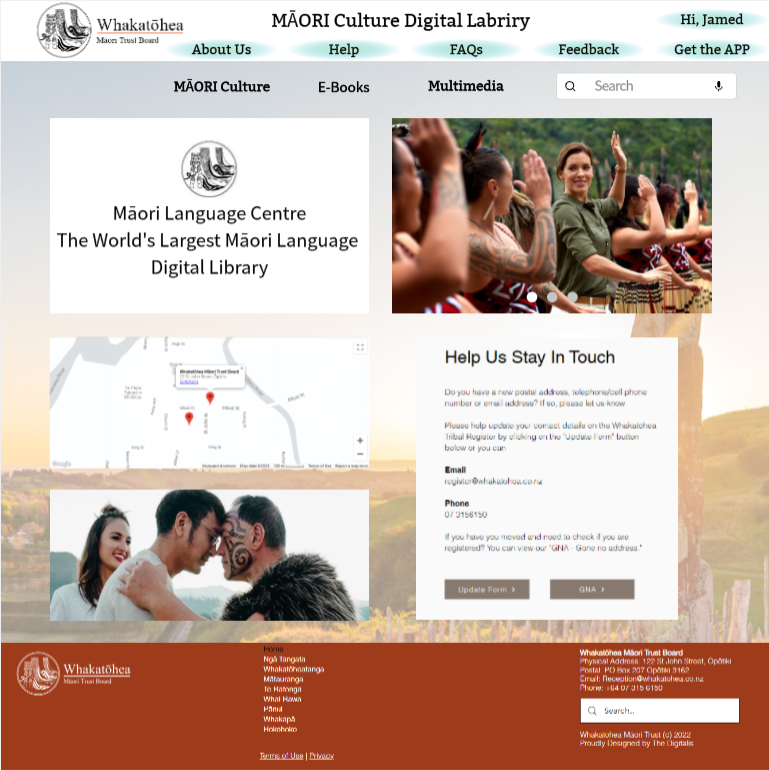
\includegraphics[width=400pt]{images/3-1-1.png}}
  \caption{Main interface}
  \label{fig30}
\end{figure}

After the user logs in, the main interface will show the Māori cultural background, the address of the Maori cultural community, the pictures of the introduction of Maori cultural activities, the links of E-books and multimedia, and the search function of the whole network. Here you can find all the resources we upload and provide, and you can also ask for help to carry out Māori language practice in the community and communicate with other Maori language learners.

\subsection{User interface}

\begin{figure}[htbp]
  \centerline{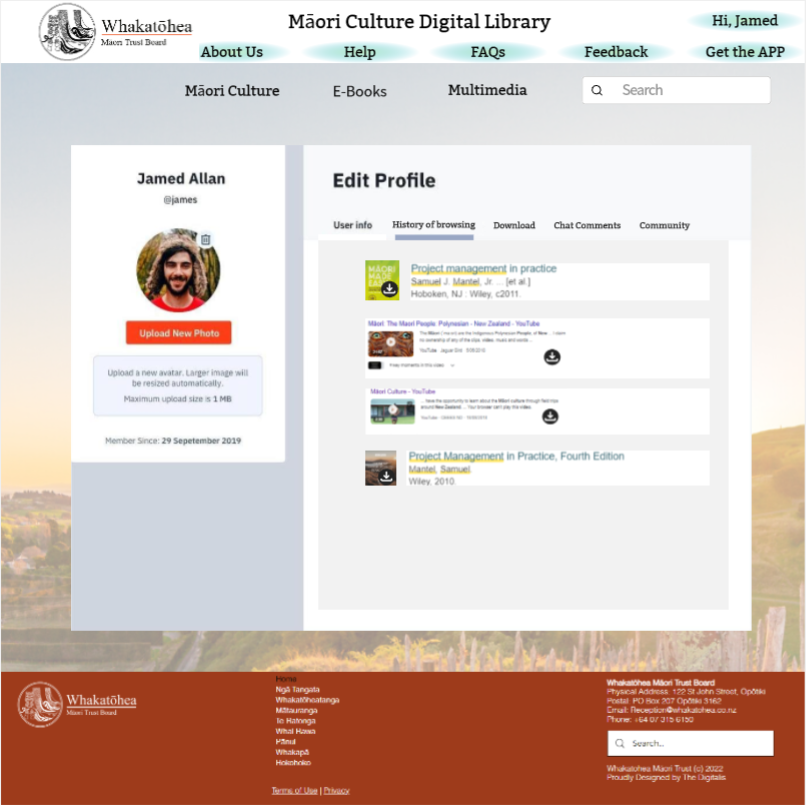
\includegraphics[width=400pt]{images/3-1-2.png}}
  \caption{User interface}
  \label{fig30}
\end{figure}

After the user logs in, The system will record user information, users can modify information through the user interface, view browsing history and like the collection of E-books or multimedia, also can communicate with friends here and view the comments of E-books or multimedia.

\subsection{Community and chat interfaces}

\begin{figure}[htbp]
  \centerline{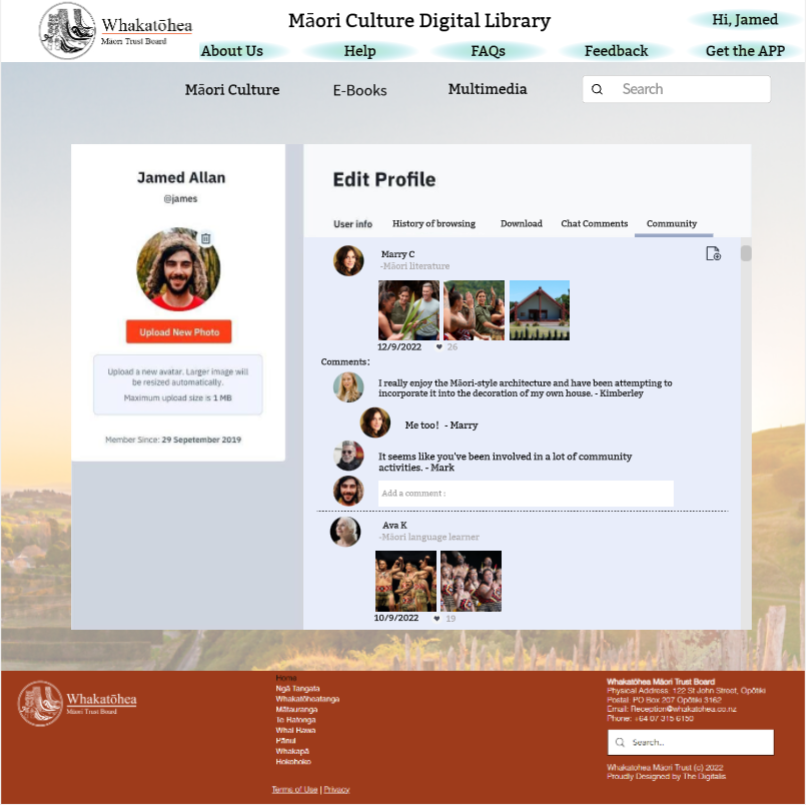
\includegraphics[width=400pt]{images/3-1-5.png}}
  \caption{Community interface}
  \label{fig30}
\end{figure}

\begin{figure}[htbp]
  \centerline{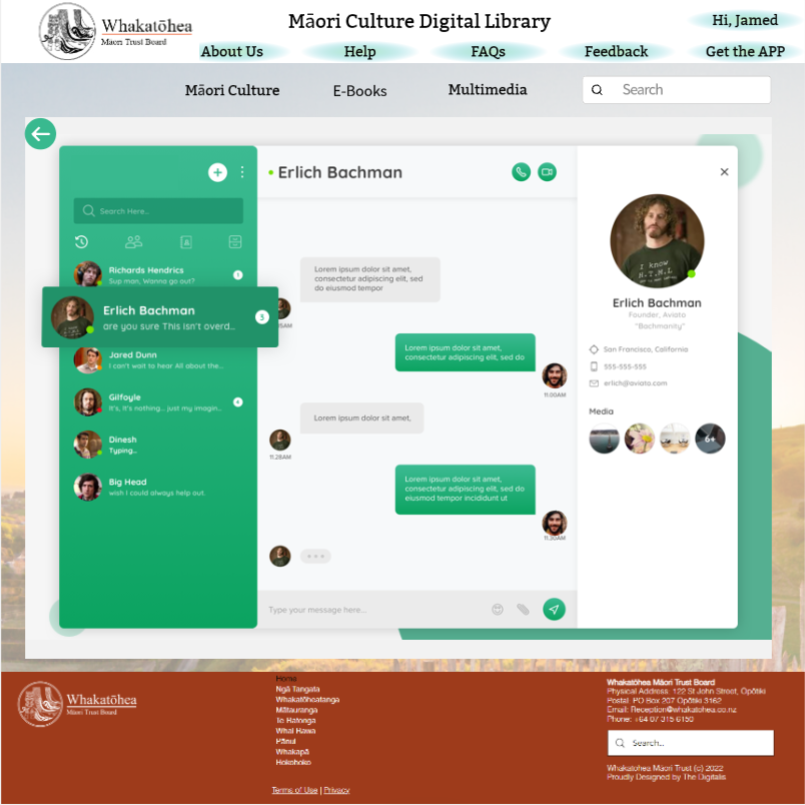
\includegraphics[width=400pt]{images/3-1-6.png}}
  \caption{Chat interface}
  \label{fig30}
\end{figure}

When users enter the user interface, they can view some public Māori activities and personal sharing in the community interface, where they can comment; When users enter the chat interface, they can communicate with netizens and share their learning results, which increases the commonality of learning.

\subsection{Māori cultural interface}

\begin{figure}[htbp]
  \centerline{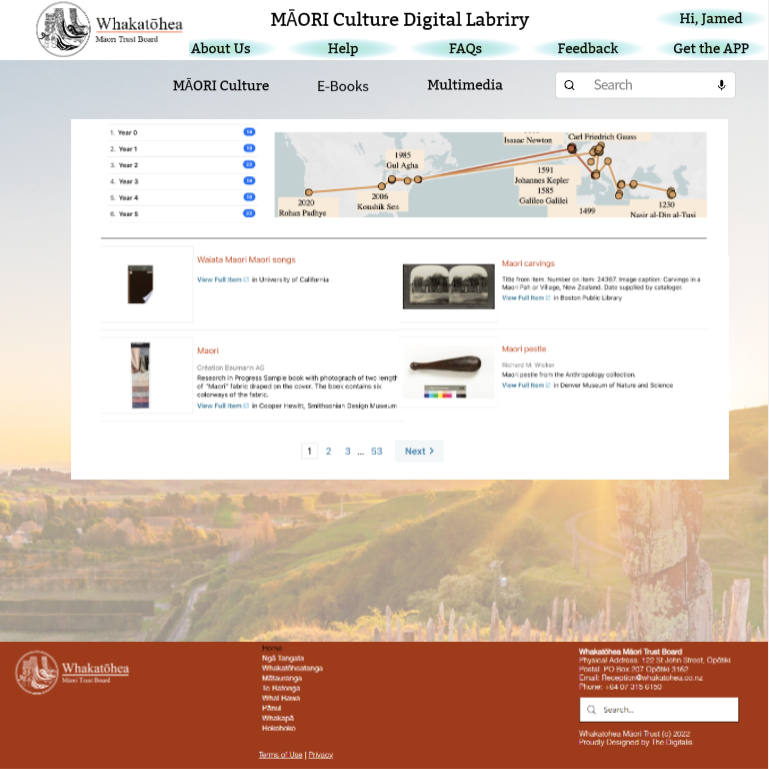
\includegraphics[width=400pt]{images/3-1-3.png}}
  \caption{Māori cultural interface}
  \label{fig30}
\end{figure}

We add a Māori culture interface where users can find all about the development process of Māori culture, migration history and distribution changes, as well as the existing Māori cultural products, which will provide more research channels for current and future learners of Māori culture, from buildings, objects to custom products to show the development process of Māori culture in all aspects\cite{MāoriCul4:online}.

\subsection{E-books browsing interface}

\begin{figure}[htbp]
  \centerline{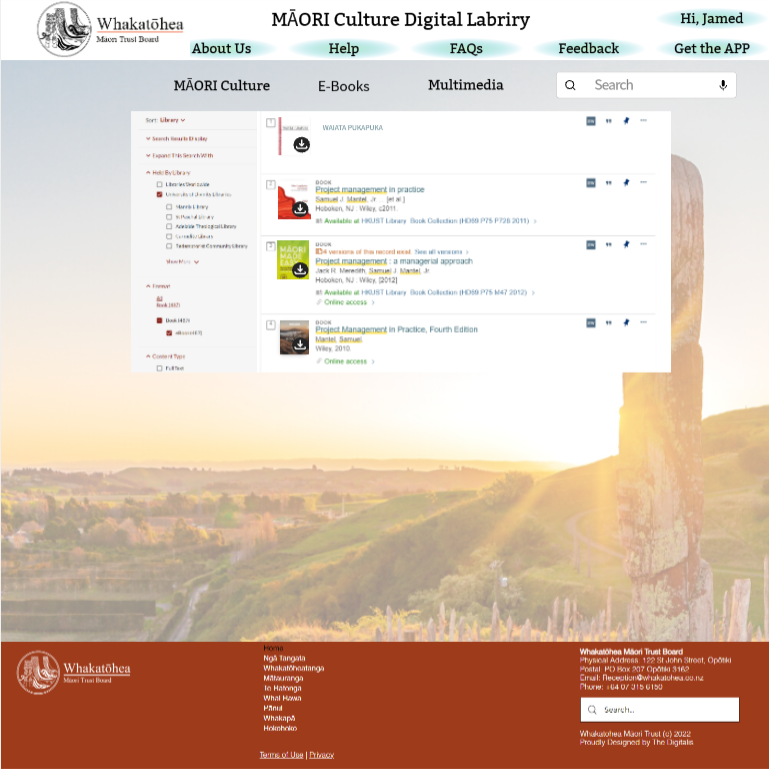
\includegraphics[width=400pt]{images/3-2-1.png}}
  \caption{E-books browsing interface}
  \label{fig30}
\end{figure}

Within the E-books browsing interface, users have the ability to search for relevant E-books using various filters. All of the filters we have designed incorporate a voice input feature, which offers convenience for learners with disabilities. Users can simply speak a keyword into the filter or apply filters from the left toolbar to display the corresponding E-books.

\subsection{The E-book interface}

\begin{figure}[htbp]
  \centerline{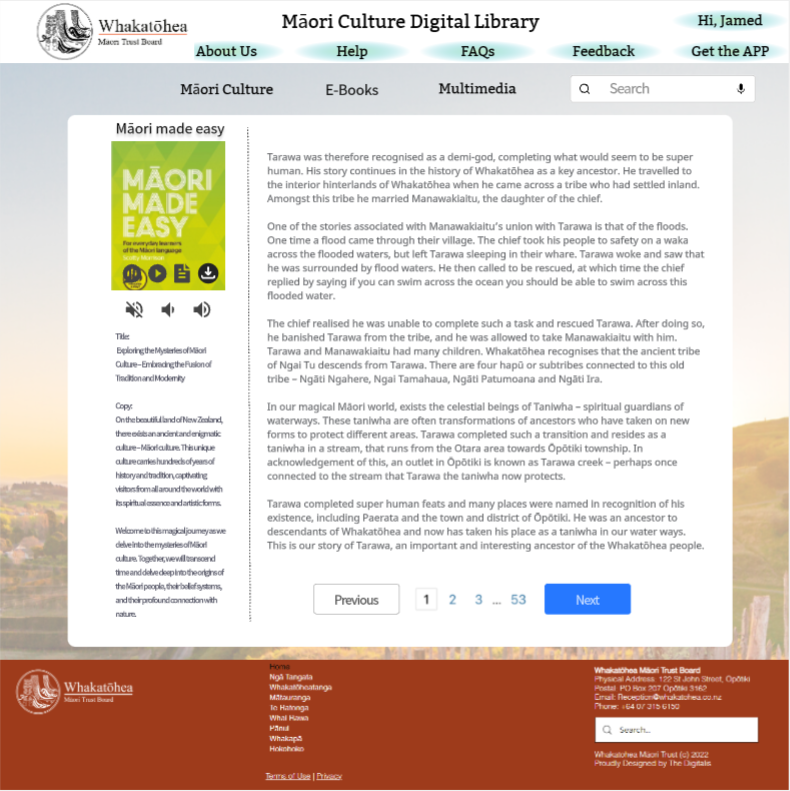
\includegraphics[width=400pt]{images/3-2-2.png}}
  \caption{The E-book interface}
  \label{fig30}
\end{figure}

In the e-book interface, the user can read the text or listen to the e-book through the voice playback function, and the translation function of other languages is provided. All resources provided by the e-library are available for download. In addition, users can complete the quiz and follow the teaching of the book through the counterattack quiz and follow the read button on this page.

\subsection{Interface of following reading }

\begin{figure}[htbp]
  \centerline{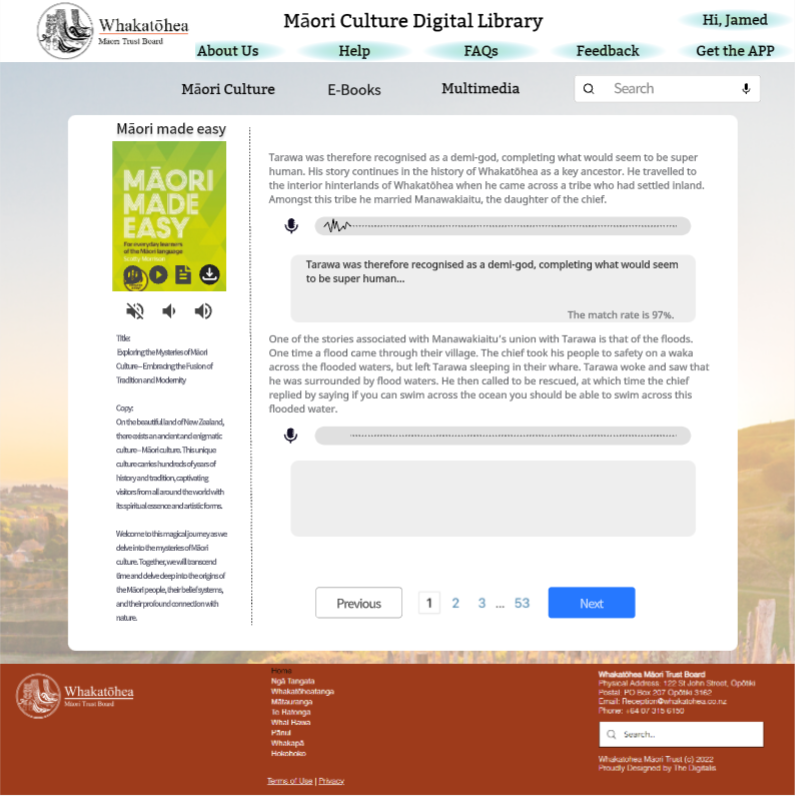
\includegraphics[width=400pt]{images/3-2-3.png}}
  \caption{The interface of following reading}
  \label{fig30}
\end{figure}

The user can enter this interface by following the reading button. In this interface, the user can play each paragraph of the book and carry out the practice of following the reading to help the user better study.

\subsection{Quiz interface}

\begin{figure}[htbp]
  \centerline{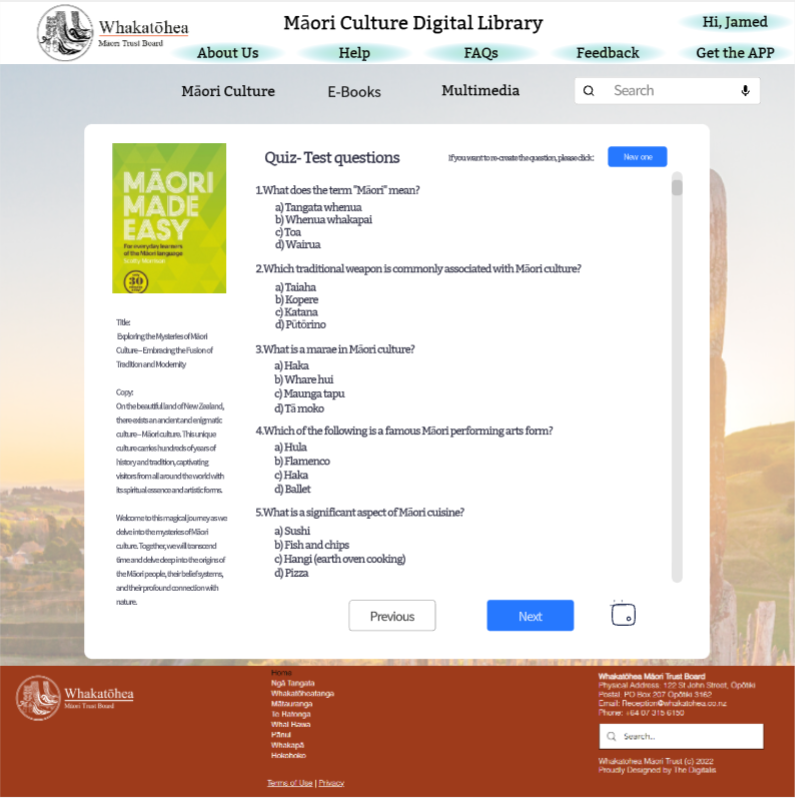
\includegraphics[width=400pt]{images/3-2-4.png}}
  \caption{Quiz interface}
  \label{fig30}
\end{figure}

Users can enter this interface through the quiz button, where they can test their learning effect. AI can randomly generate a selectable number of questions according to the content of the book, and users can test the quality of learning by themselves and deepen their understanding of the knowledge in the book.

\subsection{Video interface}

\begin{figure}[htbp]
  \centerline{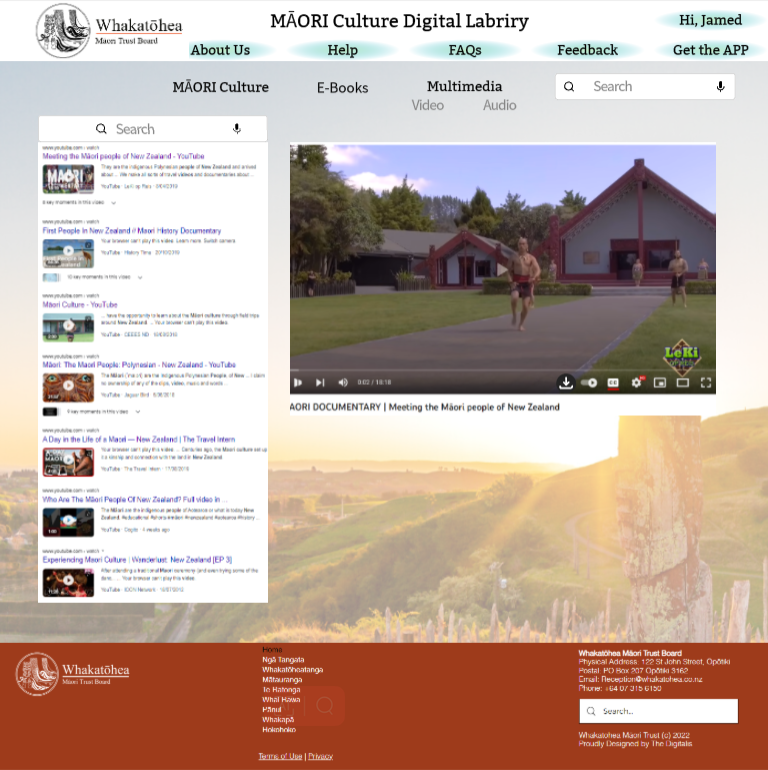
\includegraphics[width=400pt]{images/3-3-1.png}}
  \caption{Video interface}
  \label{fig30}
\end{figure}

Within the video interface, users have the capability to search for relevant videos using keywords or related terms. The filter functionality offers numerous options, including upload time, picture quality, video duration, and subtitles in other languages. These options are specifically designed to facilitate Māori learners in their viewing experience.
\subsection{Audio interface}

\begin{figure}[htbp]
  \centerline{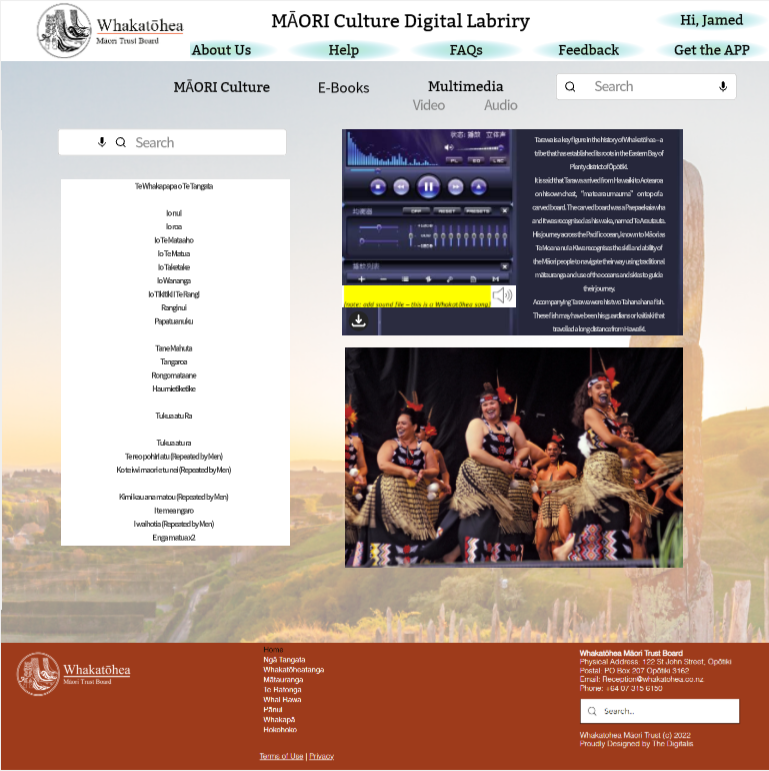
\includegraphics[width=400pt]{images/3-3-2.png}}
  \caption{Audio interface}
  \label{fig30}
\end{figure}

Within the audio interface, users have the ability to search for relevant audio files using keywords or related terms. When playing the audio files, synchronized subtitles in other languages will be displayed in the player, while the audio content itself will be displayed on the left side. This feature aims to provide convenient learning opportunities for Māori language learners. Additionally, related videos or pictures related to the audio content are displayed below, creating a favorable learning environment for audio-based learning and catering to the diverse needs of learners memory\cite{MaoriHis64:online}.

\section{Conclusion and Prospect}

Through the design and implementation of this project, the prototype design of the Māori digital library can achieve major functionalities such as book retrieval, learning, testing, and multimedia browsing. The library prototype offers a diverse range of resources pertaining to Māori culture, facilitating convenient online reading and learning for users online\cite{Māori–Te85:online}.

However, it is important to acknowledge the limitations and shortcomings of the designed prototype. Areas for improvement include optimizing the user interface design and interaction processes, enhancing the user-friendliness of the multimedia interface, and enriching the visual elements of the library frontend to cater to the learning needs of all Māori culture learners.

In conclusion, with the continuous advancement of technology and the growing Māori language community, the prototype of the digital library needs to be regularly updated and upgraded to meet the evolving needs and expectations of users. Additionally, the digital library will make a significant contribution to Māori language education and cultural preservation, fostering the inheritance and development of the Māori language, as well as promoting diverse cultural exchange and integration. Our efforts are aimed at facilitating the preservation and development of Māori culture while providing a rich and diverse platform for learning and communication. We also anticipate that the Māori digital library will become an essential learning and communication platform for Māori language users, making substantial contributions to the future development of the Māori language community community\cite{MaoriCul16:online}.

